%%%%%%%%%%%%%%%%%%%%%%%%%%%%%%%%%%%%%%%%%%%%%%%%%%%%%%%%%%%%%%%%%
% MUW Presentation
% LaTeX Template
% Version 1.0 (27/12/2016)
%
% License:
% CC BY-NC-SA 4.0 (http://creativecommons.org/licenses/by-nc-sa/3.0/)
%
% Created by:
% Nicolas Ballarini, CeMSIIS, Medical University of Vienna
% nicoballarini@gmail.com
% http://statistics.msi.meduniwien.ac.at/
%
% Customized for UAH by:
% David F. Barrero, Departamento de Automática, UAH
%%%%%%%%%%%%%%%%%%%%%%%%%%%%%%%%%%%%%%%%%%%%%%%%%%%%%%%%%%%%%%%%%

\documentclass[10pt,compress]{beamer} % Change 10pt to make fonts of a different size
\mode<presentation>

\usepackage[spanish]{babel}
\usepackage{fontspec}
\usepackage{tikz}
\usepackage{etoolbox}
\usepackage{xcolor}
\usepackage{xstring}
\usepackage{listings}

% Custom packages
\usepackage{standalone}
\usepackage{multicol}
\usepackage{multirow} % Confusion matrix
\usepackage{tikz}
\usepackage{pgfplots}
\def\layersep{2.5cm}
\usetikzlibrary{matrix,chains,positioning,decorations.pathreplacing,arrows,shapes}

\definecolor{dkgreen}{rgb}{0,0.6,0}
\definecolor{gray}{rgb}{0.5,0.5,0.5}
\definecolor{mauve}{rgb}{0.58,0,0.82}
 

\usetheme{UAH}
\usecolortheme{UAH}
\setbeamertemplate{navigation symbols}{} 
\setbeamertemplate{caption}[numbered]

%%%%%%%%%%%%%%%%%%%%%%%%%%%%%%%%%%%%%%%%%%%%%%%%%%%%%%%%%%%%%%%%%
%% Presentation Info
\title[Deep Learning]{Deep Learning}
\author{\asignatura\\\carrera}
\institute{}
\date{Departamento de Automática}
%%%%%%%%%%%%%%%%%%%%%%%%%%%%%%%%%%%%%%%%%%%%%%%%%%%%%%%%%%%%%%%%%


%%%%%%%%%%%%%%%%%%%%%%%%%%%%%%%%%%%%%%%%%%%%%%%%%%%%%%%%%%%%%%%%%
%% Descomentar para habilitar barra de navegación superior
\setNavigation
%%%%%%%%%%%%%%%%%%%%%%%%%%%%%%%%%%%%%%%%%%%%%%%%%%%%%%%%%%%%%%%%%

%%%%%%%%%%%%%%%%%%%%%%%%%%%%%%%%%%%%%%%%%%%%%%%%%%%%%%%%%%%%%%%%%
%% Configuración de logotipos en portada
%% Opacidad de los logotipos
\newcommand{\opacidad}{1}
%% Descomentar para habilitar logotipo en pié de página de portada
\renewcommand{\logoUno}{Images/isg.png}
%% Descomentar para habilitar logotipo en pié de página de portada
%\renewcommand{\logoDos}{Images/CCLogo.png}
%% Descomentar para habilitar logotipo en pié de página de portada
%\renewcommand{\logoTres}{Images/ALogo.png}
%% Descomentar para habilitar logotipo en pié de página de portada
%\renewcommand{\logoCuatro}{Images/ELogo.png}
%%%%%%%%%%%%%%%%%%%%%%%%%%%%%%%%%%%%%%%%%%%%%%%%%%%%%%%%%%%%%%%%%

%%%%%%%%%%%%%%%%%%%%%%%%%%%%%%%%%%%%%%%%%%%%%%%%%%%%%%%%%%%%%%%%%
%% FOOTLINE
%% Comment/Uncomment the following blocks to modify the footline
%% content in the body slides. 


%% Option A: Title and institute
\footlineA
%% Option B: Author and institute
%\footlineB
%% Option C: Title, Author and institute
%\footlineC
%%%%%%%%%%%%%%%%%%%%%%%%%%%%%%%%%%%%%%%%%%%%%%%%%%%%%%%%%%%%%%%%%


% This is for the confusion matrix, DELETE if not needed
\def\colorModel{hsb} %You can use rgb or hsb

\newcommand\ColCell[1]{
   \pgfmathparse{#1<50?1:0}  %Threshold for changing the font color into the cells
       \ifnum\pgfmathresult=0\relax\color{white}\fi
   \pgfmathsetmacro\compA{0}      %Component R or H
   \pgfmathsetmacro\compB{#1/100} %Component G or S
   \pgfmathsetmacro\compC{1}      %Component B or B
   \edef\x{\noexpand\centering\noexpand\cellcolor[\colorModel]{\compA,\compB,\compC}}\x #1
} 
%\newcolumntype{E}{>{\collectcell\ColCell}m{0.4cm}<{\endcollectcell}}  %Cell width
\newcommand*\rot{\rotatebox{90}}


\begin{document}

%%%%%%%%%%%%%%%%%%%%%%%%%%%%%%%%%%%%%%%%%%%%%%%%%%%%%%%%%%%%%%%%%
% Use this block for a blue title slide with modified footline
{\titlepageBlue
    \begin{frame}
        \titlepage
    \end{frame}
}

\institute{\asignatura}

\begin{frame}[plain]{}
   \begin{block}{Objectives}
      \begin{enumerate}
         \item Define Machine Learning (ML)
		 \item Delimite ML scope
         \item Introduce the main ML tasks
         \item Recognize problems as ML tasks
      \end{enumerate} 
   \end{block}

   \begin{block}{Bibliography}
	\begin{itemize}
        \item Bishop, Christopher M. \textit{Pattern Recognition and Machine Learning}. 2nd edition. Springer-Verlag. 2011
        \item M\"uller, Andreas C., Guido, Sarah. \textit{Introduction to Machine Learning with Python}. O'Reilly. 2016
	\end{itemize}
   \end{block}
\end{frame}

{
\disableNavigation{white}
\begin{frame}[shrink]{Table of Contents}

 	\frametitle{Table of Contents}
  	\begin{multicols}{2}
  		\tableofcontents
    \end{multicols}

 %\frametitle{Table of Contents}
 %\tableofcontents
  % You might wish to add the option [pausesections]
\end{frame}
}

\subsection{Deep neural networks}

\begin{frame}{Algorithms}{Deep neural networks (I)}
     Deep Learning is not just a network with many layers
	\begin{itemize}
		\item Gradient vanishing
		\item Multiple local optima -> difficult training
	\end{itemize}

	\centering
	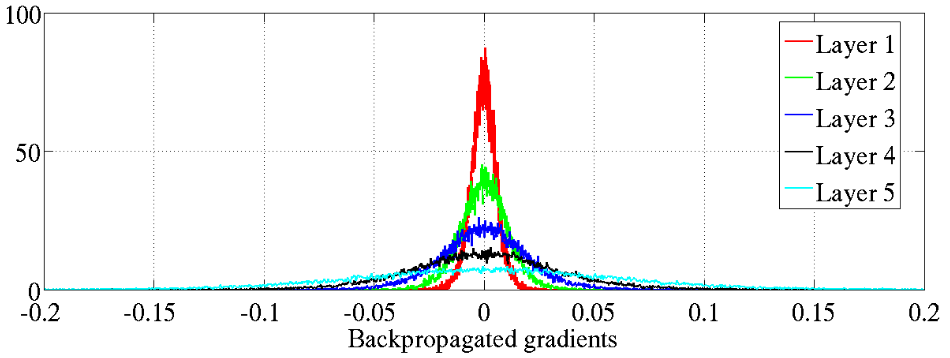
\includegraphics[width=0.6\textwidth]{figs/gradients.png}\\
	\scriptsize\href{http://proceedings.mlr.press/v9/glorot10a/glorot10a.pdf?source=post\_page---------------------------}{(Source)}\\

	\normalsize
	\flushleft
	Usual solutions
	\begin{itemize}
		\item Careful weights initialization
		\item ReLU and Leaky ReLU activation functions
		\item Regularization through \alert{dropout}
	\end{itemize}
\end{frame}

\begin{frame}{Algorithms}{Deep neural networks (II)}
	Two popular types of deep networks
	\begin{itemize}
		\item Convolutional Neural Networks (CNNs)
		\item Long Short-Term Memory (LSTM) 
		\item ... we use both
	\end{itemize}

	In Deep Learning, we think in layers \\

	\centering
	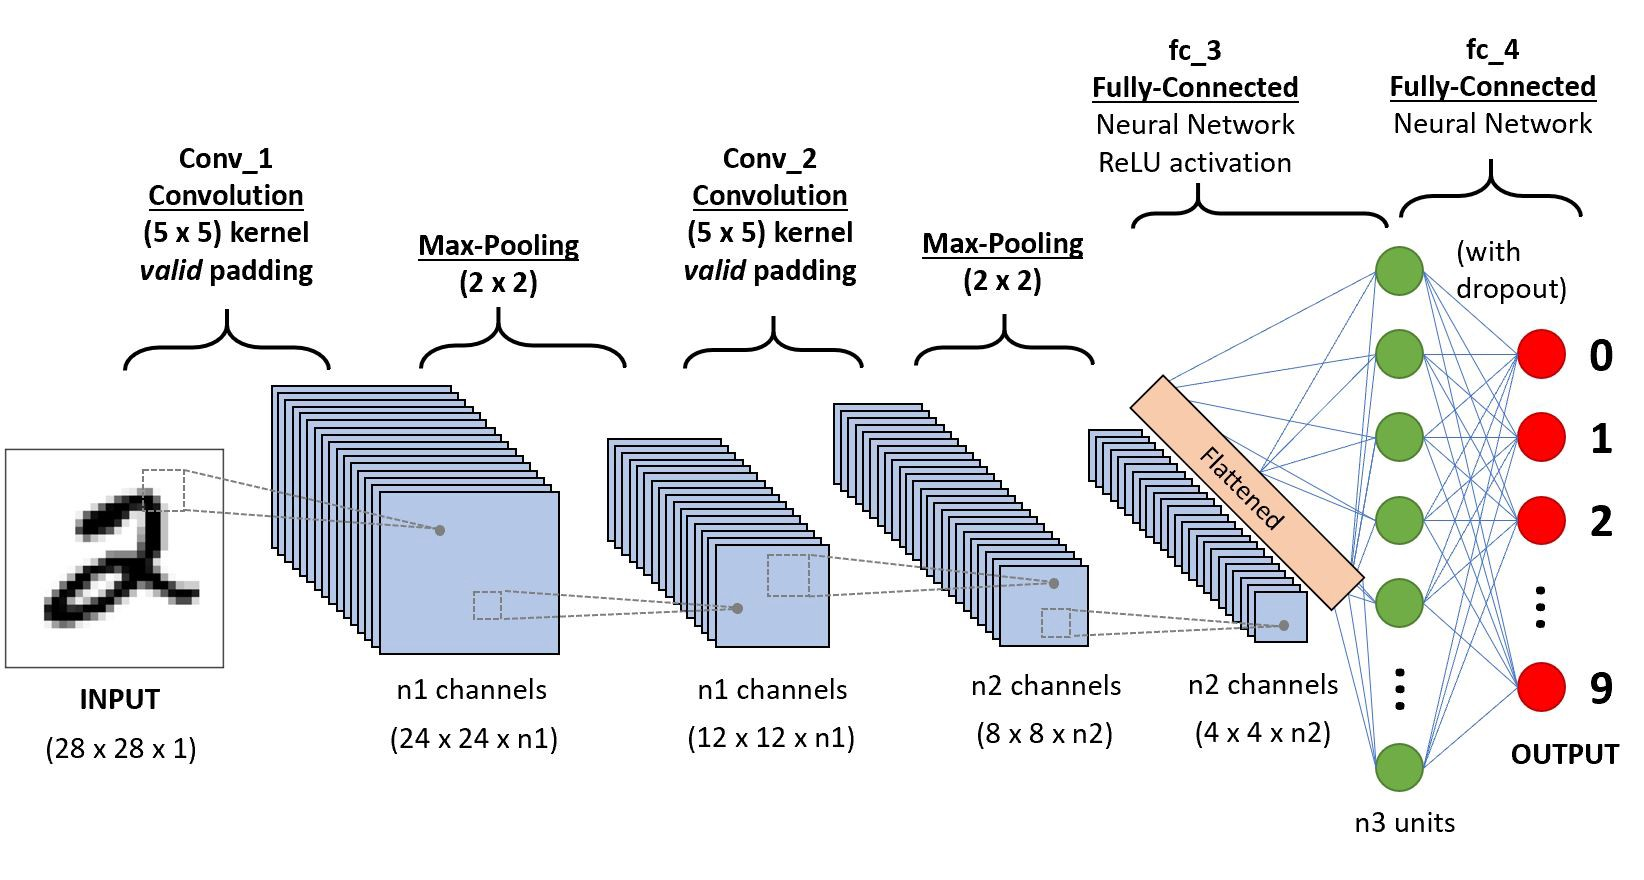
\includegraphics[width=0.7\textwidth]{figs/layers.png}\\
	\scriptsize\href{https://towardsdatascience.com/a-comprehensive-guide-to-convolutional-neural-networks-the-eli5-way-3bd2b1164a53}{(Source)}\\

	\end{frame}

\subsection{1D convolution}

\begin{frame}{Algorithms}{1D convolution}
        CNNs are popular for Computer Vision applications
	\begin{itemize}
		\item Networks with convolutional layers
		\item Convolutions in NN use to be 2D
		\item \href{https://miro.medium.com/max/500/1*GcI7G-JLAQiEoCON7xFbhg.gif}{(Conv 2D example)}
	\end{itemize}

	Univariable time series are 1D
	\begin{itemize}
		\item \alert{1D convolution}
	\end{itemize}

	\centering
	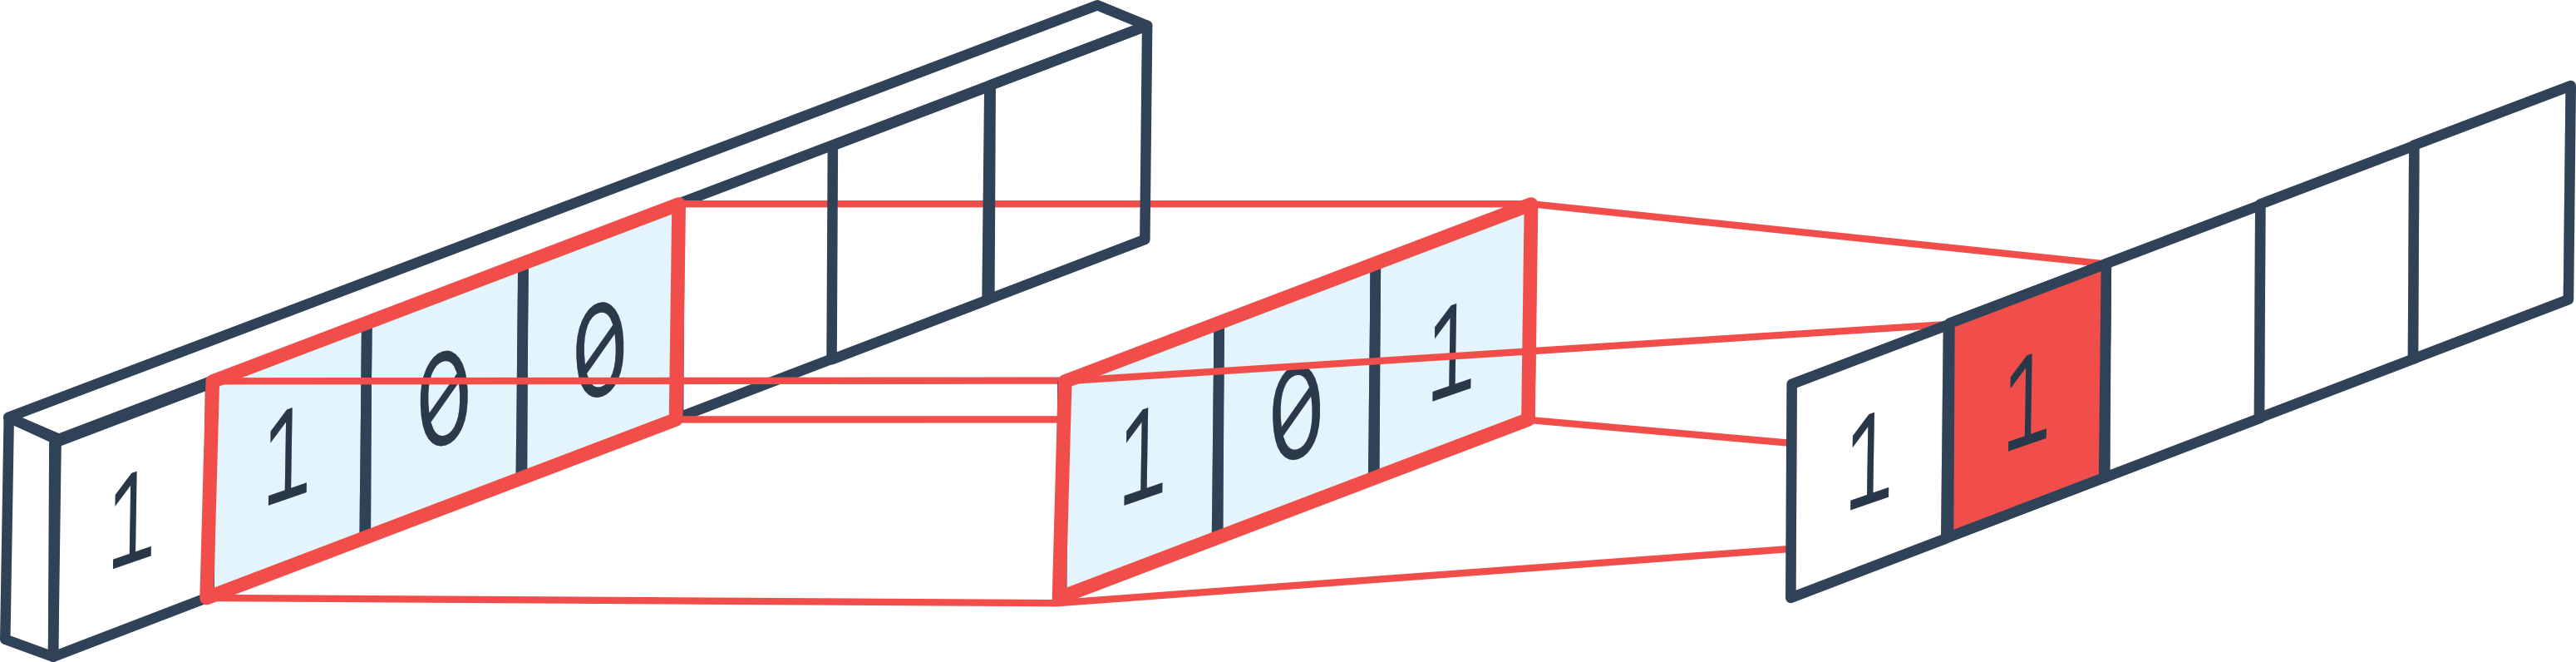
\includegraphics[width=0.5\textwidth]{figs/1dconv.png}

    	\flushleft Related concept: \alert{deconvolution} \\
\end{frame}

\subsection{Max-pooling}

\begin{frame}{Algorithms}{Max-pooling}
     	Max-pooling down-samples data instances
	\begin{itemize}
		\item Given a matrix, it takes its maximum value
		\item Usually the matrix is $n x n$ (2D)
	\end{itemize}
	Benefits
	\begin{itemize}
		\item Dimensionality reduction
		\item Filters irrelevant information
	\end{itemize}
	\bigskip
	\centering 
	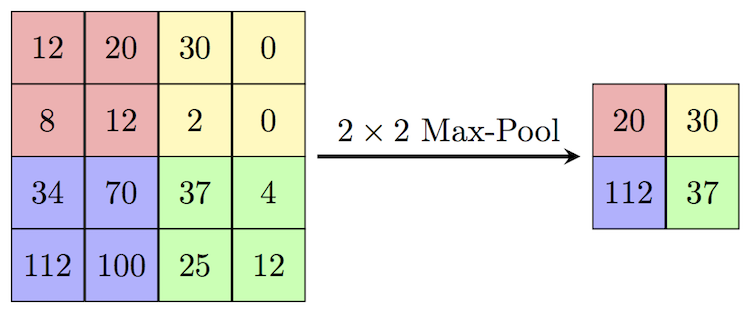
\includegraphics[width=0.5\textwidth]{figs/maxpool.png}
\end{frame}

\subsection{Dropout}

\begin{frame}{Algorithms}{Dropout}
	\alert{Dropout} is a regularization technique for neural networks
	\begin{itemize}
		\item Dropout deactivates a neuron with probability $p$ for each iteration
	\end{itemize}

	Related concept: \alert{dense layers}
	\begin{itemize}
		\item In Keras, it is just a fully connected layer with regular neurons
	\end{itemize}

	\centering
        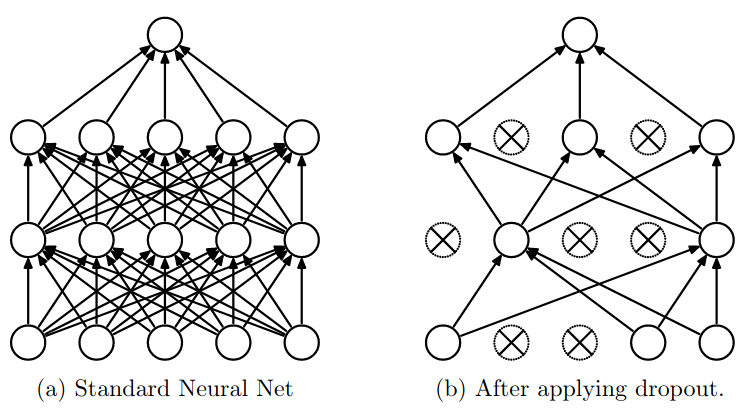
\includegraphics[width=0.6\textwidth]{figs/dropout.png}\\
	\scriptsize\href{https://jmlr.org/papers/volume15/srivastava14a.old/srivastava14a.pdf}{(Srivastava et al. (2010))}
\end{frame}


\subsection{LSTM networks}

\begin{frame}{LSTM networks}{Recurrent neural networks}
    TODO
\end{frame}

\begin{frame}{LSTM networks}{LSTM}
    TODO
\end{frame}

\section{Autoencoders}

\subsection{Autoencoders}

\begin{frame}{Autoencoders}{Autoencoders}
	\centering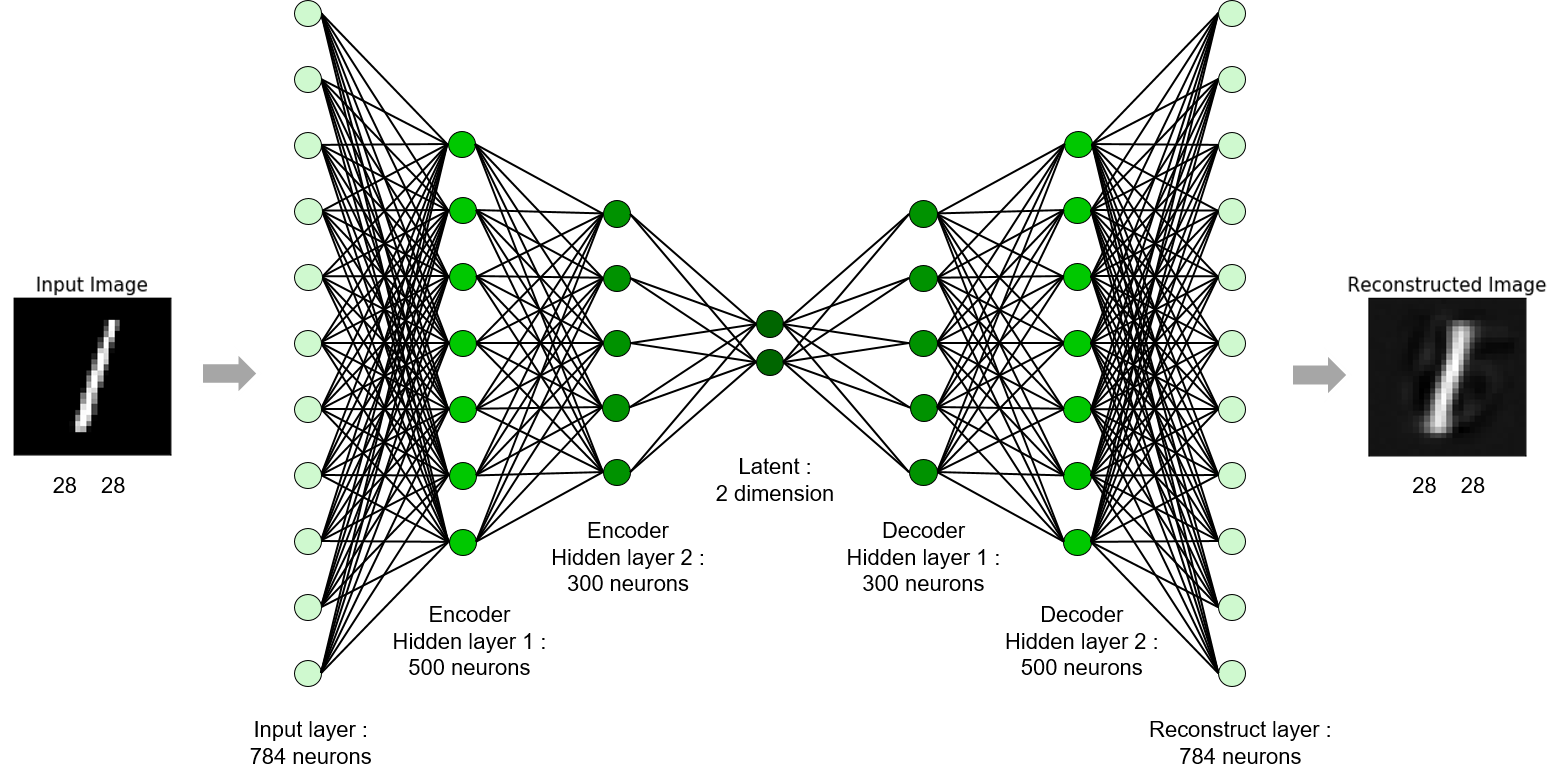
\includegraphics[width=0.75\linewidth]{figs/autoencoder.png}\\
	\centering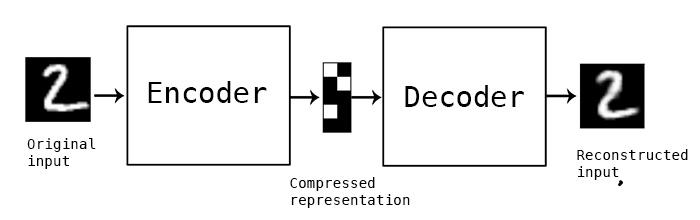
\includegraphics[width=0.3\linewidth]{figs/autoencoder2.png}\\
	\scriptsize\href{http://i-systems.github.io/HSE545/machine\%20learning\%20all/KIMM/06\_KIMM\_Autoencoder.html}{(Source)}
	\medskip

	\normalsize

	\begin{flushleft}
	Important concepts: \alert{latent space} and \alert{latent variables}
	\end{flushleft}
\end{frame}

\subsection{Autoencoders for anomaly detection}

\begin{frame}{Autoencoders}{Autoencoders for anomaly detection (I)}
	\documentclass[crop,tikz]{standalone}% 'crop' is the default for v1.0, before it was 'preview'

\usetikzlibrary{shapes,arrows}

\begin{document}


\tikzstyle{block} = [draw, rectangle, minimum height=3em, minimum width=6em]
\tikzstyle{sum} = [draw, circle, node distance=1cm]
\tikzstyle{input} = [coordinate]
\tikzstyle{output} = [coordinate]
\tikzstyle{pinstyle} = [pin edge={to-,thin,black}]

\begin{tikzpicture}[auto, node distance=2cm,>=latex']
 \node [input, name=input] {};
 \coordinate [right of=input, node distance=1.5cm] (sum){};
 %\node [sum, right of=input] (sum) {};
 \node [block, right of=sum] (autoencoder) {Autoencoder};
 \node [sum, right of=autoencoder, node distance=2.5cm] (resta) {$-$};
 \node [input, name=output, right of=resta, node distance = 2cm] {$-$};
 \coordinate [below of=autoencoder, node distance=1.5cm] (abajo){};
 %\node [block, right of=controller, node distance=3cm] (motor) {G$_{motor}$};
 %\node [block, right of=motor, pin={[pinstyle]above:Störningar},
 %       node distance=3cm] (system) {Dynamik$_{\varphi}$};

 %\draw [->] (controller) -- node[name=u] {$u$} (motor);
 %\node [output, right of=system] (output) {};
 %\node [block, below of=motor] (msystem) {Mätsystem};

	\draw [draw,->] (input) -- node {$\vec{x}$} (autoencoder);
 %\draw [->] (sum) -- node {$e$} (autoencoder);
	\draw [->] (autoencoder) -- node {$\vec{x}'$} (resta);
	\draw [->] (resta) -- node {$\epsilon$} (output);
	%\draw [->] (resta) -- node {$\epsilon=||\vec{x}'-\vec{x}'$||} (output);
	\draw [->] (sum) |- (abajo) -| (resta);
 %\draw [|-] (sum) -- node {} (abajo);
 %\draw [-|] (abajo) -- node {} (resta);

 %\draw [->] (system) -- node [name=y] {$\varphi$}(output);
 %\draw [->] (y) |- (msystem);
 %\draw [->] (msystem) -| node[pos=0.99] {$-$}  node [near end] {$\varphi_m$} (sum);
\end{tikzpicture}

\end{document} 

	\bigskip
	\alert{Reconstruction error} is an anomality measure
	\begin{itemize}
		\item A norm can be computed to provide a global measure (MAE/MSE), or ...
		\item ... keep reconstruction error as vector
	\end{itemize}
    PCA may be used, less powerfull than autoencoders
\end{frame}

\begin{frame}{Autoencoders}{Autoencoders for anomaly detection (II)}
	\centering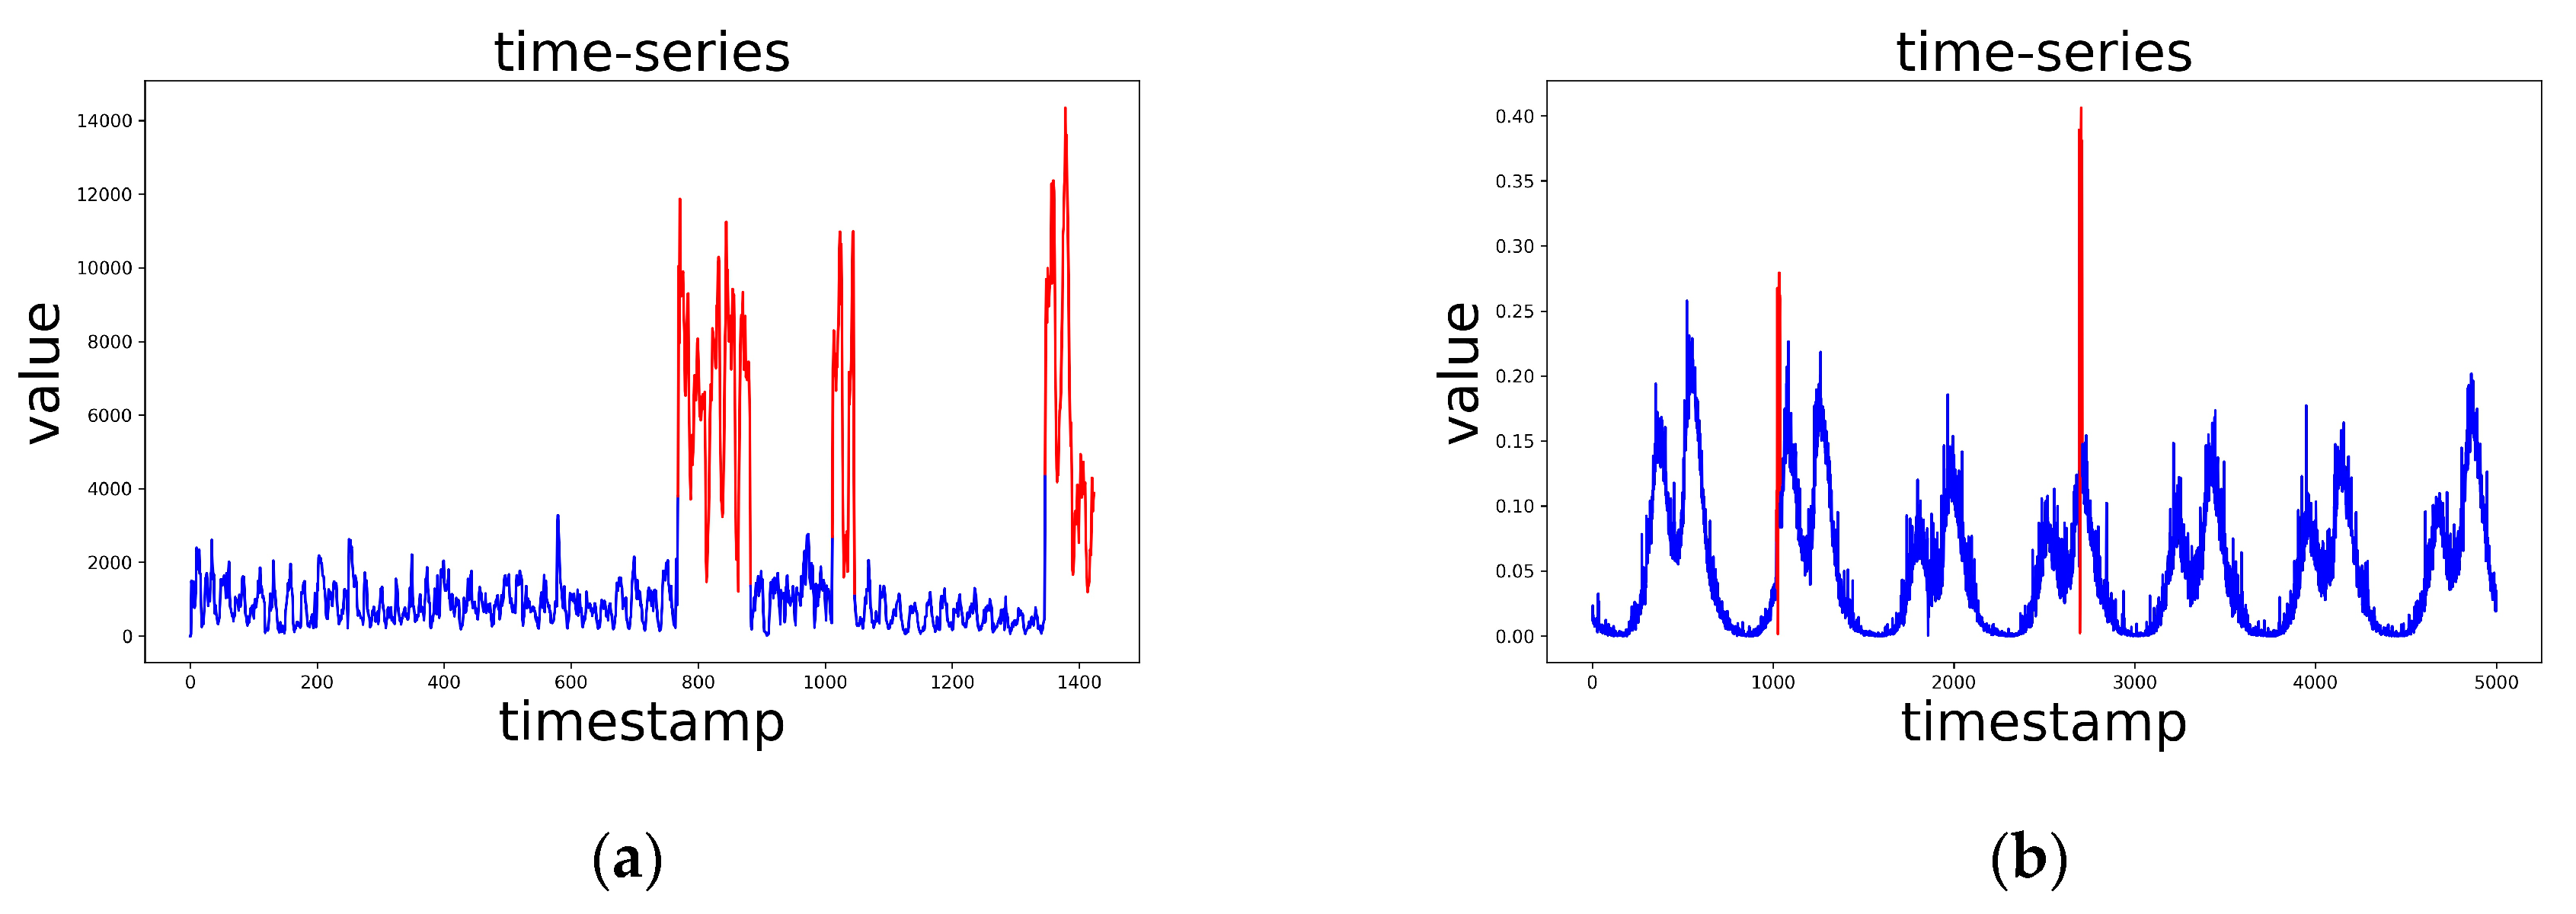
\includegraphics[width=0.75\linewidth]{figs/autoencoderts.png}\\
	\scriptsize\href{https://www.mdpi.com/1424-8220/20/13/3738}{(Source: Niu, Z.; Yu, K.; Wu, X. \textit{LSTM-Based VAE-GAN for Time-Series Anomaly Detection}. Sensors 2020, 20, 3738.)}

	\bigskip
	\begin{flushleft}
	\normalsize{
	Great flexibility to handle reconstruction error
	\begin{itemize}
		\item Trigger an alarm based on a threshold
		\item Analize the time-series
		\item Feed a classifier
	\end{itemize}
	}
	\end{flushleft}
\end{frame}

\subsection{Autoencoders as generative models}
\begin{frame}{Autoencoders}{Autoencoders as generative models (I)}
    \begin{columns}
 	   \column{.60\textwidth}
     Any autoencoder may be used as a generative model
	\begin{itemize}
		\item The decoder can reconstruct an instance from a latent space sample
	\end{itemize}

 	   \column{.40\textwidth}
	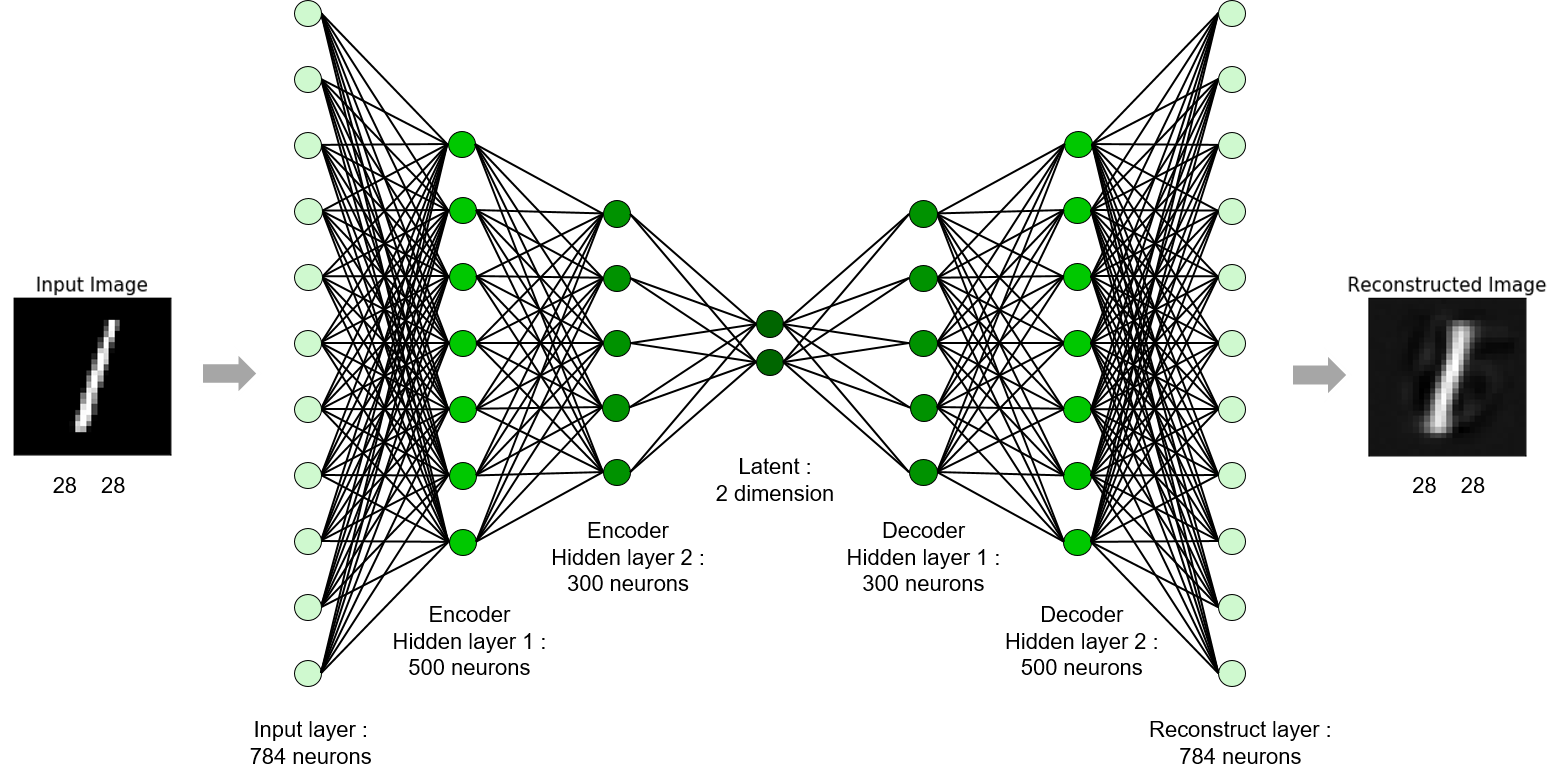
\includegraphics[width=\textwidth]{figs/autoencoder.png}\\
	\scriptsize\href{http://i-systems.github.io/HSE545/machine\%20learning\%20all/KIMM/06\_KIMM\_Autoencoder.html}{(Source)}
		
	\end{columns}

	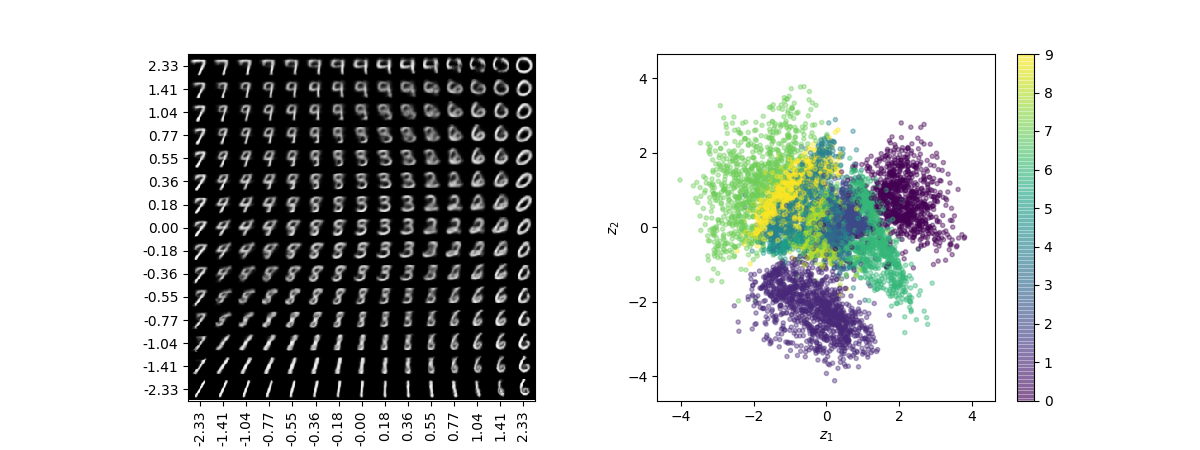
\includegraphics[width=\textwidth]{figs/latent2.png}\\
	\scriptsize\href{https://towardsdatascience.com/intuitively-understanding-variational-autoencoders-1bfe67eb5daf}{(Source)}
\end{frame}

\begin{frame}{Autoencoders}{Autoencoders as generative models (II)}
	Regular autoencoders are not a good choice for generative models

    \begin{columns}
 	   \column{.40\textwidth}
		\begin{figure}
	        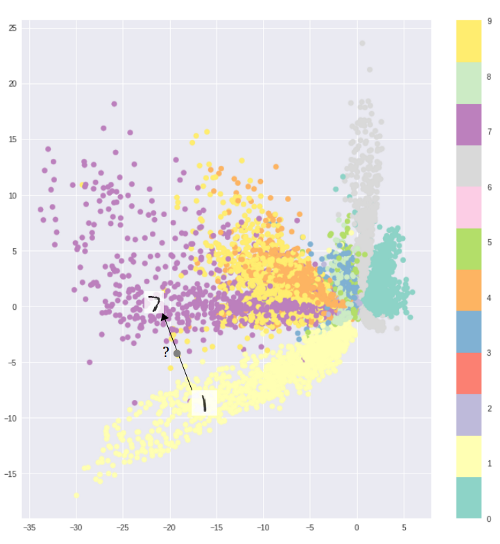
\includegraphics[width=\textwidth]{figs/latent.png}\\
		\scriptsize\href{https://towardsdatascience.com/intuitively-understanding-variational-autoencoders-1bfe67eb5daf}{(Source)}
		\end{figure}
    \end{columns}

\end{frame}


\section{Advanced topics}

\subsection{Variational autoencoders}

\begin{frame}{Advanced topics}{Variational Autoencoders (I)}
	\centering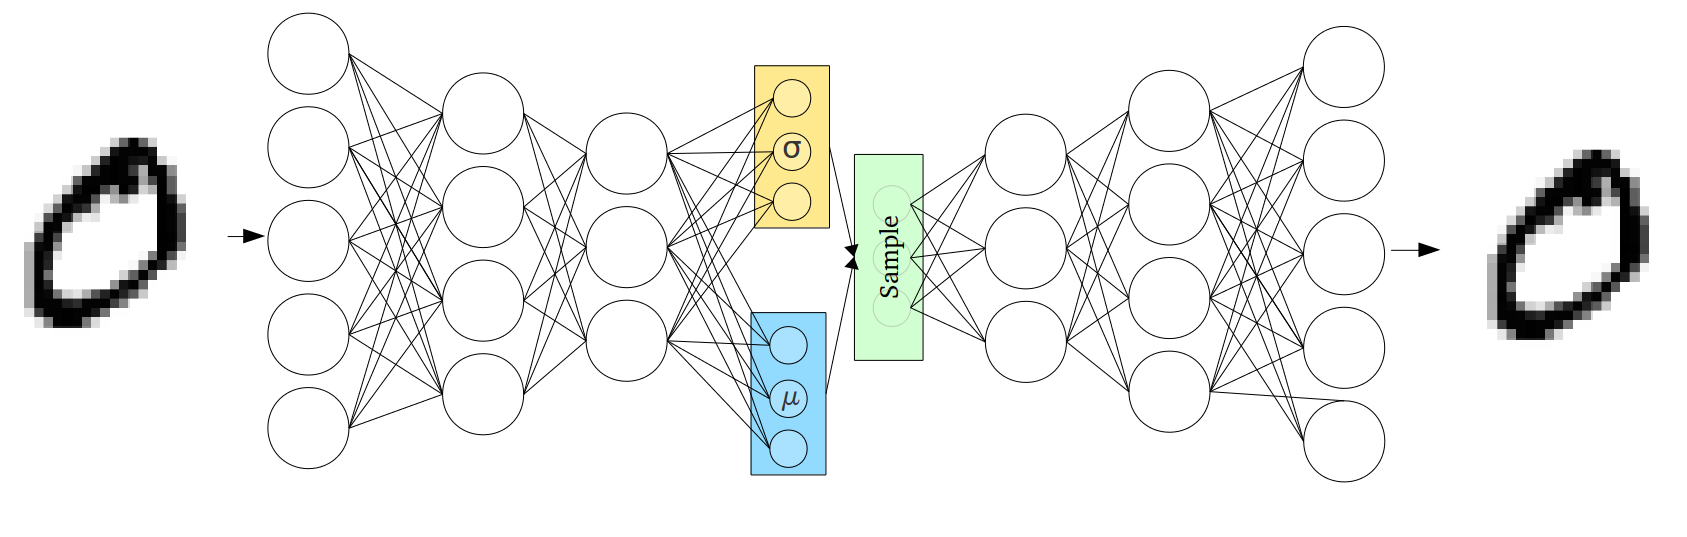
\includegraphics[width=0.85\linewidth]{figs/vae.png}\\
	\scriptsize\href{https://towardsdatascience.com/intuitively-understanding-variational-autoencoders-1bfe67eb5daf}{(Source)}

	\bigskip

	\flushleft
	\normalsize

	VAEs encodes latent variables as probability distributions
	\begin{itemize}
		\item Gaussian distributions with $\mu$ and $\sigma$
		\item Decoder sample the distributions
	\end{itemize}
\end{frame}

\begin{frame}{Advanced topics}{Variational Autoencoders (II)}
	\centering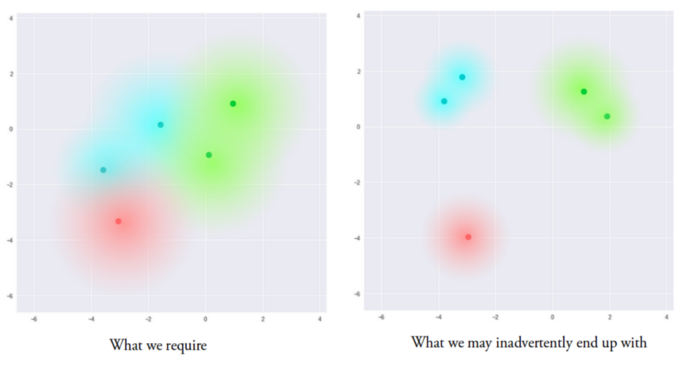
\includegraphics[width=0.6\linewidth]{figs/vae-kl.png}\\
	\scriptsize\href{https://towardsdatascience.com/intuitively-understanding-variational-autoencoders-1bfe67eb5daf}{(Source)}

	\smallskip

	\flushleft
	\normalsize

	We want a structured latent space
	\begin{itemize}
		\item Penalty based on \textit{Kullback-Leibler} (KL) divergence
			\begin{itemize}
				\item KL measures divergente between two probability distributions
			\end{itemize}
	\end{itemize}
\end{frame}


\subsection{VAE semantics}

\begin{frame}{Advanced topics}{VAE semantics (I)}
	Astonishing VAE feature: latent space has semantics!
	\centering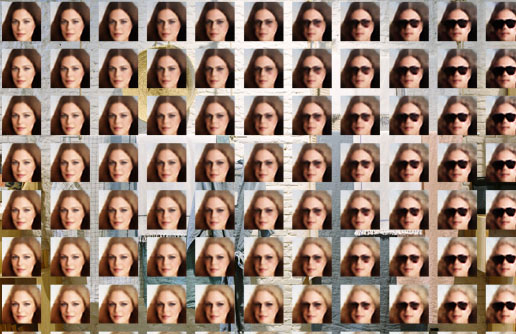
\includegraphics[width=0.7\linewidth]{figs/faces.jpg}\\
	\scriptsize\href{https://www.compthree.com/blog/autoencoder/}{(Source)}

\end{frame}

\begin{frame}{Advanced topics}{VAE semantics (II)}
	Another incredible VAE property: 'semantic' arithmetic operations
	\centering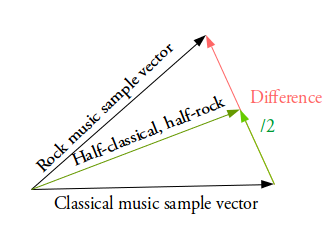
\includegraphics[width=0.3\linewidth]{figs/vector-vae1.png}\quad
	\centering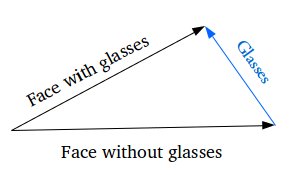
\includegraphics[width=0.3\linewidth]{figs/vector-vae2.png}\\
	\scriptsize\href{https://towardsdatascience.com/intuitively-understanding-variational-autoencoders-1bfe67eb5daf}{(Source)}
\end{frame}

\begin{frame}{Advanced topics}
    GANs\\
    VAEs\\
    Adversarial examples
\end{frame}


\end{document}
